\lecture{7}{19 marzo 2024}
\section{Studio di un'onda progressiva}

Studiamo ora il caso generico di una forza applicata alla sorgente dell'onda su una corda. (Finora abbiamo studiato un moto noto sulla sorgente, non una forza generica).

\begin{figure}[H]
	\centering
	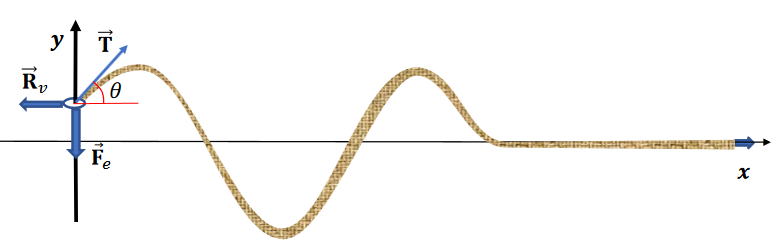
\includegraphics[width=0.8\textwidth]{screenshots/2024-03-19-11-12-22.png}
	\caption{Schema della corda studiata.}
	\label{fig:corda-forzata}
\end{figure}

Impostando l'equazione della dinamica per il moto dell'anello posto in \(x=0\) otteniamo:
\[
	\vec{F_e} + \vec{T} +\vec{R_v}  = \mathrm{d}m \vec{a} \rightsquigarrow \begin{dcases}
		T\cos \theta + R_v = \mathrm{d} m a_x\\
		F_y + T\sin \theta =\mathrm{d} m a_y  \\
	\end{dcases}
\]

Facendo tendere \(\mathrm{d} m \to 0\), i membri di destra tendono a zero.
\[
	\begin{dcases}
		T\cos \theta + R_v = 0\\
		F_y + T\sin \theta = 0  \\
	\end{dcases}
	\rightsquigarrow F_y = -T\sin \theta \thickapprox -T \tan \theta = -T \frac{\partial \xi }{\partial x}
\]
Di conseguenza \(F_y = -T \left. \frac{\partial \xi }{\partial x}\right\vert_x=0 \). In questo sistema si producono esclusivamente onde progressive (\(f(x-vt)\)), se ci fosse un + al posto del - tratteremmo invece onde regressive.
\begin{figure}[H]
	\centering
	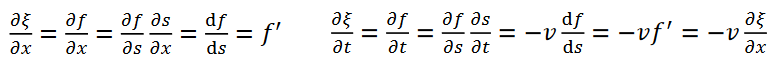
\includegraphics[width=0.8\textwidth]{screenshots/2024-03-19-11-22-13.png}
\end{figure}
Per quanto scritto sopra,
\[
	\frac{\partial \xi }{\partial x} = - \frac{1}{v} \frac{\partial \xi }{\partial t} \rightsquigarrow F_y(t) = \frac{T}{v}\frac{\partial \xi (0,t)}{\partial t} 
\]
La derivata parziale di \(\xi \) calcolata nel punto 0 rappresenta la velocità verticale del punto sorgente, che verrà indicata con \(v_c(t)\). Inoltre possiamo definire l'impedenza meccanica della corda.
\begin{definition}
	[Impedenza meccanica]
	Si definisce impedenza meccanica:
	\[
		Z=\frac{T}{v}= T \sqrt{\frac{\mu }{T}} = \sqrt{\mu T}  
	\]
\end{definition} 
L'effetto della forzante è quindi quello di mettere in moto il primo punto della corda con una velocità proporzionale alla forza (di solito non è così!):
\[
	F_y(t) = Zv_c(t)
\]
Usare \(v\) e \(Z\) al posto di T e \(\mu \) ci permetterà di trovare risultati molto più generali.

\paragraph{C'è una forza viscosa?}

Sembra che nel sistema ci sia una forza viscosa che porta la forza a essere proporzionale alla velocità. Si possono interpretare le formule come se la corda fosse in grado di applicare una forza dipendente dalla velocità: \(F_v(t) = -Z v_c(t)\). L'energia non viene dissipata, è assorbita e utilizzata per mettere in moto punti sempre più lontani della corda.

\begin{note}
	\(v_c(t)\) è sempre in fase con la forzante, quindi siamo sistematicamente in una situazione di risonanza.
\end{note}

\subsection{Energia e potenza}

Il lavoro compiuto dalla forzante è \(\delta L = \vec{F} \cdot \mathrm{d} \vec{s} = F_y \mathrm{d} y = F_y \frac{\mathrm{d}\xi }{\mathrm{d}t} \mathrm{d} t = F_y v_c \mathrm{d} t \). Tuttavia, per quanto ricavato prima so che

\begin{figure}[H]
	\centering
	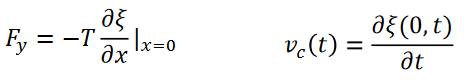
\includegraphics[width=0.45\textwidth]{screenshots/2024-03-19-11-33-56.png}
\end{figure}

E la potenza risulta quindi:
\[
	\mathcal{P} = \frac{\delta L}{\mathrm{d} t} = -T \left. \frac{\partial \xi }{\partial x} \right\vert_{x=0} \left. \frac{\partial \xi}{\partial t}\right\vert_{x=0} 
\]
Tuttavia la relazione è più generale e vale per ogni punto della corda:
\[
	\mathcal{P} = -T \frac{\partial \xi }{\partial x} \frac{\partial \xi }{\partial t}
\]
Per le onde progressive sappiamo già che 
\begin{figure}[H]
	\centering
	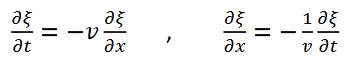
\includegraphics[width=0.5\textwidth]{screenshots/2024-03-19-11-37-15.png}
	\caption{Relazione fra la derivata temporale e spaziale per le onde progressive.}
	\label{fig:dt-dx-onda-prog}
\end{figure}
Di conseguenza la potenza può essere riscritta:
\begin{gather*}
	\mathcal{P} (x,t) = \frac{T}{v}\left(\frac{\partial \xi (x,t)}{\partial t}\right)^{2}  = Tv\left(\frac{\partial \xi (x,t)}{\partial x} \right)^{2} \\
	\mathcal{P} (x,t) = Z \left(\frac{\partial \xi (x,t)}{\partial t}\right)^{2}
\end{gather*}
Si vede subito che la potenza è sempre maggiore o uguale a zero. Quanto ricavato è valido in generale per tutte le onde meccaniche.

\paragraph{Energia cinetica}
Consideriamo un tratto di corda infinitesima in moto con velocità \(v=\frac{\partial \xi }{\partial t} \). 
\begin{figure}[H]
	\centering
	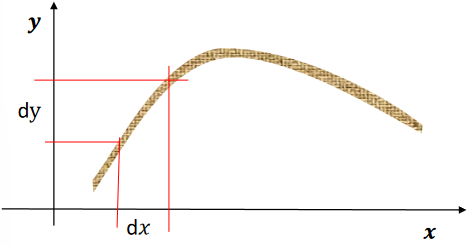
\includegraphics[width=0.6\textwidth]{screenshots/2024-03-19-11-44-58.png}
	\caption{L'immagine di riferimento per lo studio di energia cinetica e potenziale sulla corda.}
	\label{fig:energia-corda}
\end{figure}
Ottengo che 
\[
	\mathrm{d} K = \frac{1}{2} \mathrm{d} m v ^{2} = \frac{1}{2} \mu \left( \frac{\partial \xi }{\partial t}  \right) ^{2} \mathrm{d} x
\]
Da cui posso definire una densità lineare di energia cinetica:
\[
	u_K(x,t) = \frac{\mathrm{d}K}{\mathrm{d}x} = \frac{1}{2} \mu \left( \frac{\partial \xi }{\partial t}  \right) ^{2} 
\]

\paragraph{Energia potenziale}

Si fa riferimento sempre alla \autoref{fig:energia-corda}. Il tratto infinitesimo di corda viene allungato facendo lavoro contro la tensione della corda: \(\delta L = -T (\mathrm{d}l - \mathrm{d} x ) = -T(\sqrt{\mathrm{d}x^{2} + \mathrm{d} y ^{2}   } - \mathrm{d} x )\). Applicando l'approssimazione delle piccole oscillazioni otteniamo che
\begin{gather*}
	\delta L = -T \mathrm{d} x \left( \sqrt{1+ \left( \frac{\partial \xi }{\partial x}  \right)^{2}  } -1  \right) \thickapprox -T \mathrm{d} x \left( 1+\frac{1}{2} \left( \frac{\partial \xi }{\partial x}  \right)^{2} + \cdots - 1  \right) \thickapprox \\
	\thickapprox -\frac{1}{2}T \left( \frac{\partial \xi }{\partial x}  \right)^{2} \mathrm{d} x\\
	u_P(x,t) = -\frac{\delta L}{\mathrm{d} x} = \frac{1}{2}T\left( \frac{\partial \xi }{\partial x}  \right) ^{2} 
\end{gather*}
Dove nell'ultima riga abbiamo definito la densità di energia potenziale.

\paragraph{Energia meccanica}
Possiamo definire la densità di energia meccanica:
\begin{definition}
	[Densità lineare di energia meccanica]
	\[
		u(x,t) = \frac{1}{2} \mu \left( \frac{\partial \xi }{\partial t}  \right) ^{2} + \frac{1}{2}T\left( \frac{\partial \xi }{\partial x}  \right) ^{2}
	\]
\end{definition}
Nel caso di onde progressive abbiamo le formule già viste che collegano la derivata in x alla derivata in t (\autoref{fig:dt-dx-onda-prog}), quindi possiamo ricavare la seguente uguaglianza:
\begin{figure}[H]
	\centering
	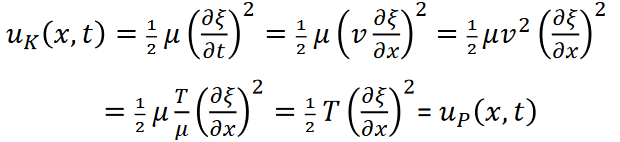
\includegraphics[width=0.6\textwidth]{screenshots/2024-03-19-11-56-45.png}
\end{figure}
L'energia potenziale e l'energia cinetica sono uguali istante per istante in ogni punto! Quindi l'energia totale è il doppio dell'energia cinetica e il doppio dell'energia potenziale. La potenza e l'energia trasmessa sono inoltre proporzionali:
\begin{figure}[H]
	\centering
	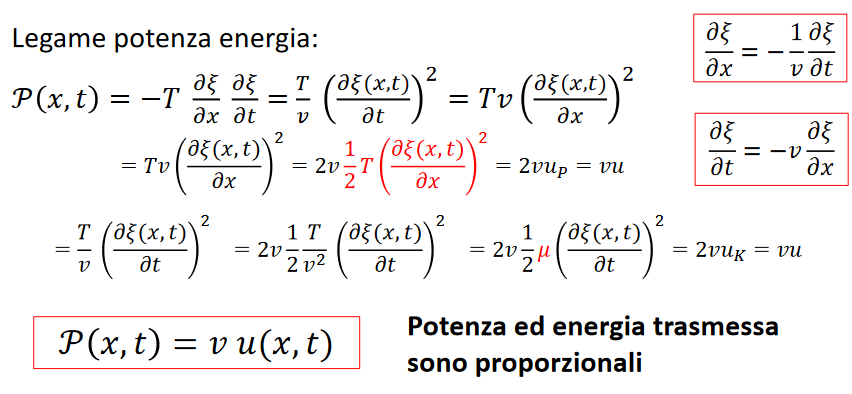
\includegraphics[width=0.7\textwidth]{screenshots/2024-03-19-11-58-19.png}
\end{figure}

\subsection{Scambi di energia}
Si fa riferimento alla \autoref{fig:corda-forzata}. L'energia immessa dalla forzante serve ad indurre un'onda nella corda e viene incamerata dalla corda nella sua forma (è il ruolo della forza viscosa). Quindi l'energia raccolta da ogni elemento della corda viene persa passandola all'elemento di corda adiacente! Questo trasporto di energia è necessario per mettere in moto elementi lontani della corda dove l'onda non è ancora arrivata.

\begin{eg}
	Consideriamo una semicorda omogenea (con tensione T e densità di massa \(\mu \)) il cui estremo è sottoposto al moto \(\xi (0,t) = -A \sin \omega t = A \sin (-\omega t)\), che produce un'onda progressiva: \(\xi (x,t) = A \sin (kx - \omega t)\).
	\begin{figure}[H]
		\centering
		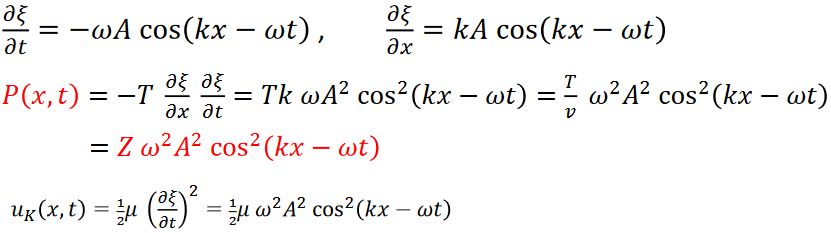
\includegraphics[width=0.8\textwidth]{screenshots/2024-03-19-12-20-11.png}
	\end{figure}
	Ritrovo inoltre quanto già visto, ovvero che energia cinetica ed energia potenziale sono istante per istante, punto per punto, uguali.
	\begin{figure}[H]
		\centering
		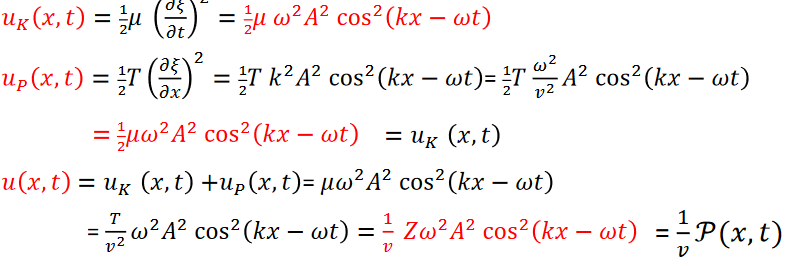
\includegraphics[width=0.8\textwidth]{screenshots/2024-03-19-12-22-16.png}
	\end{figure}
	Tutte le forme di energia appena ricavate dipendono da \(kx-\omega t\)! Quindi esse sono soluzioni delle equazioni di D'Alembert.
	\begin{align}
		\frac{\partial ^{2} \mathcal{P} (x,t)}{\partial x^{2} } &= \frac{1}{v^{2} }\frac{\partial ^{2} \mathcal{P} (x,t)}{\partial t^{2} }
		&
		\frac{\partial ^{2} u (x,t)}{\partial x^{2} } &= \frac{1}{v^{2} }\frac{\partial ^{2} u(x,t)}{\partial t^{2} }  
	\end{align}
\end{eg}
Quanto trovato ora è valido per ogni onda meccanica, sia regressiva che progressiva! Ogni volta che ho un'onda meccanica ho delle onde di potenza e delle onde di densità lineare di energia meccanica.
\begin{figure}[H]
	\centering
	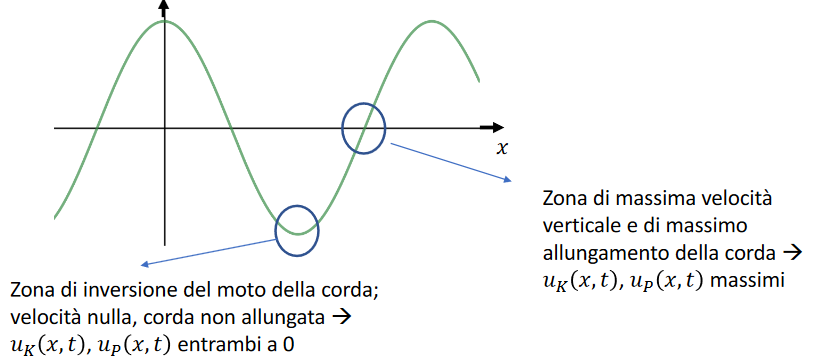
\includegraphics[width=0.8\textwidth]{screenshots/2024-03-19-12-26-23.png}
	\caption{Conseguenze della dipendenza di \(u_K\) e \(u_P\) da \((kx-\omega t)\).}
\end{figure}

\subsection{Trasporto di energia e potenza}
Le onde meccaniche trasportano energia e potenza, come appena accennato. Ricaviamo la potenza e l'energia media:
\begin{figure}[H]
	\centering
	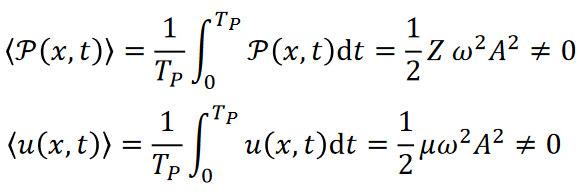
\includegraphics[width=0.5\textwidth]{screenshots/2024-03-19-12-28-50.png}
\end{figure}
Ricordiamo che invece lo spostamento medio (in cui non compare l'oscillazione elevata al quadrato) è nullo: \(\langle \xi (x,t)\rangle  = \frac{1}{T_P} \int_{0}^{T_P} \xi (x,t)rm  \,\mathrm{d}t =0\).
Le formule ricordano quelle dell'oscillatore armonico: dipendenza dal quadrato dell'ampiezza e dal quadrato della pulsazione.
\paragraph{Energia trasmessa in un periodo}
Ricordando che \(\mathcal{P} (x,t) = Z \omega ^{2} A ^{2} \cos ^{2} (kx-\omega t)\),
\begin{figure}[H]
	\centering
	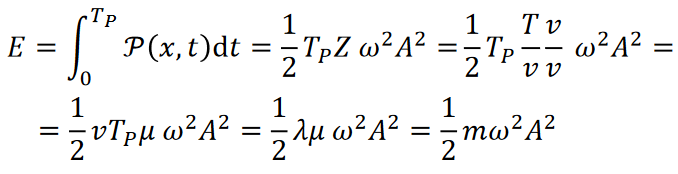
\includegraphics[width=0.6\textwidth]{screenshots/2024-03-19-12-32-43.png}
\end{figure}
Ho ritrovato la formula dell'oscillatore armonico per l'energia presente in un tratto di corda lungo \(\lambda: E = \frac{1}{2}m \omega ^{2} A^{2}  \), ovvero in un periodo \(T_P\).

\subsection{Intensità}

Si definisce l'intensità dell'onda meccanica.

\begin{definition}
	[Intensità]\label{def:intensita}
	Per le onde periodiche, si definisce l'intensità dell'onda:
	\[
		I = \frac{E(\Delta t)}{\Delta t} = \frac{1}{T_P}\int_{0}^{T_P} \mathcal{P} (x,t) \,\mathrm{d}r = \langle \mathcal{P}  \rangle = \left\langle Z \left( \frac{\partial \xi (x,t)}{\partial t} \right)^{2}   \right\rangle 
	\]
	\(I\) è misurata in watt.
\end{definition}

Per una singola onda armonica si ritrova il risultato già visto: \(I = \langle \mathcal{P}  \rangle = \frac{1}{2}Z \omega ^{2} A ^{2} \). Se l'onda è periodica può essere scritta in serie di Fourier, che per le onde periodiche progressive (N.B.: non scriviamo \(a_0\) perché nel calcolo della potenza compaiono solo derivate e quindi questo termine costante non ha rilevanza) è
\begin{figure}[H]
	\centering
	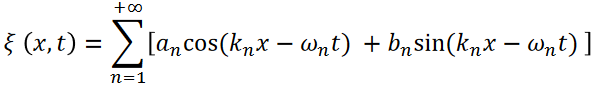
\includegraphics[width=0.6\textwidth]{screenshots/2024-03-19-12-40-52.png}
\end{figure}
Che permette di ricavare un'espressione dell'intensità come serie analoga a quanto visto per una singola onda (N.B.: restano solo i termini \(\sin (k_n x- \omega _n t) \sin (k_m x- \omega _m t)\) e \(\cos (k_n x- \omega _n t) \cos (k_m x- \omega _m t)\)) con \(m=n\):
\begin{figure}[H]
	\centering
	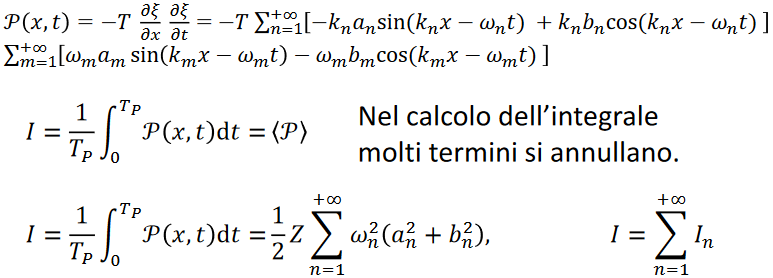
\includegraphics[width=0.7\textwidth]{screenshots/2024-03-19-12-42-32.png}
\end{figure}
Dove è stato posto \(I_n = \frac{1}{2} Z \omega ^{2} _n (a^{2} _n + b ^{2} _n )\). Questo ci permette di rappresentare lo spettro di potenza dell'onda in funzione della pulsazione, perché \(I_n\) è funzione di \(\omega _n\).

\begin{note}
	Domande tipiche da orale:
	\begin{itemize}
		
		\item Perché non si definisce l'intensità per onde impulsive?
		\item Quale grandezza fisica potrebbe sostituire l'intensità per le onde impulsive?
		\item Qual è l'espressione dello spettro di potenza se uso la serie complessa di Fourier?
	\end{itemize}
\end{note}